
%(BEGIN_QUESTION)
% Copyright 2011, Tony R. Kuphaldt, released under the Creative Commons Attribution License (v 1.0)
% This means you may do almost anything with this work of mine, so long as you give me proper credit

In this process, maple syrup is heated as it passes through a steam heat exchanger, then enters an evaporator where the water boils off.  The purpose of this is to raise the sugar concentration of the syrup, making it suitable for use as a food topping.  A level control system (LT, LIR, LIC, and LV) maintains constant syrup level inside the evaporator, while an analytical control system (AT, AIR, AIC, and AV) monitors the sugar concentration of the syrup and adjusts steam flow to the heat exchanger accordingly.

$$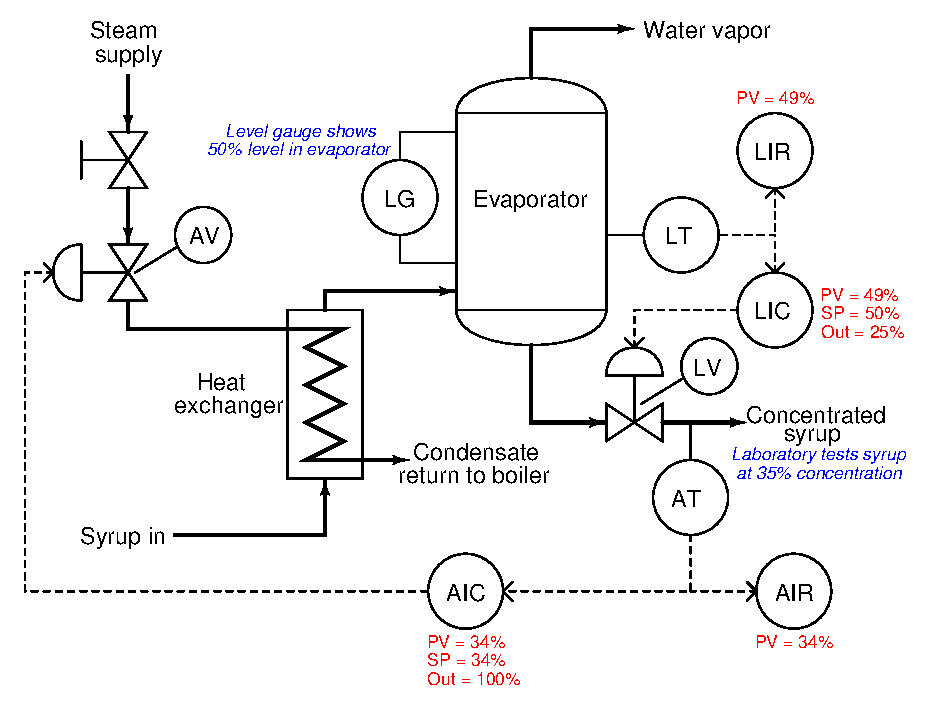
\includegraphics[width=15.5cm]{i04132x01.eps}$$

Examine the variable values shown in the above diagram, and then determine where any problems may exist in this syrup concentrating system.  Also, describe the first test, measurement, or observation you would perform to diagnose the problem, and how this first step would inform your next diagnostic step.

\vskip 20pt \vbox{\hrule \hbox{\strut \vrule{} {\bf Suggestions for Socratic discussion} \vrule} \hrule}

\begin{itemize}
\item{} Although this process seems rather tame, can you think of any places where we might wish to install {\it process safety} equipment or instrumentation to help avoid a process emergency?
\end{itemize}

\underbar{file i04132}
%(END_QUESTION)





%(BEGIN_ANSWER)


%(END_ANSWER)





%(BEGIN_NOTES)

Tha major problem here seems to be that the concentration controller output is saturated at 100\%.  It should not have to ``work this hard'' to achieve setpoint!

A good first test would be to inspect the AV stem position, to see if it is really at 100\% open.  If so, then there is a mechanical problem somewhere (not enough steam; clogged exchanger; shut hand valve?).  If not, then there is a problem somewhere between the controller and the control valve.

\vfil \eject

\noindent
{\bf Summary Quiz:}

Identify a diagnostic {\it test} or {\it meausurement} you would make in this system after observing its symptoms:

$$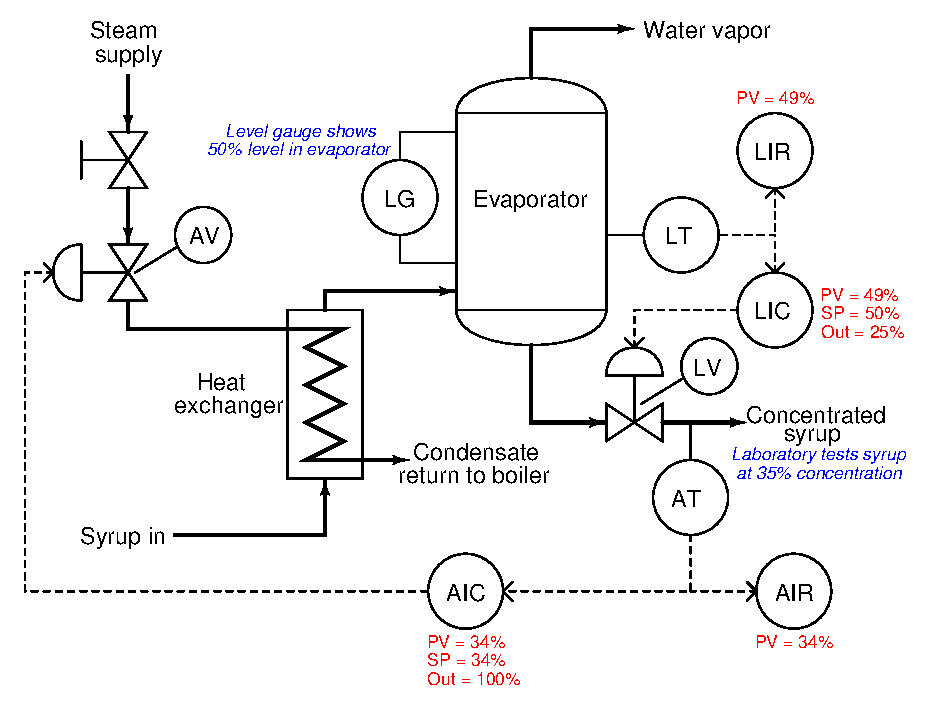
\includegraphics[width=15.5cm]{i04132x01.eps}$$

%INDEX% Basics, control loop troubleshooting
%INDEX% Process: maple syrup concentration (single-effect evaporator)

%(END_NOTES)


